\vspace{1cm}

\section{Memoization and dynamic programming}
\label{sec:memo-dynam-progr}

Recursive code tends to be simple and clear, but sometimes it is
highly inefficient. Think of the method that we wrote before to
calculate the n$^{th}$ Fibonacci number: 

\begin{verbatim}
    public static int fib(int n) {
        if ((n == 1) || (n == 2)) {
          return 1; 
        } else {
            int result = fib(n-1) + fib(n-2);
            return result;
        }
    }
\end{verbatim}

This methods works fine for small numbers (up to 30), but then it
becomes extremely expensive to compute and takes a very long to
provide an answer, as shown in Figure~\ref{fig:fibotime}. Why is this? 

\begin{figure}[hbtp]
  \centering
  %
% This LaTeX code paints an exponential curve:
%
%   x: n
%   y: time to calculate fibonacci(n) naively
%
%
% GNUPLOT: LaTeX picture
\setlength{\unitlength}{0.240900pt}
\ifx\plotpoint\undefined\newsavebox{\plotpoint}\fi
\sbox{\plotpoint}{\rule[-0.200pt]{0.400pt}{0.400pt}}%
\begin{picture}(1500,900)(0,0)
\sbox{\plotpoint}{\rule[-0.200pt]{0.400pt}{0.400pt}}%
\put(211.0,131.0){\rule[-0.200pt]{4.818pt}{0.400pt}}
\put(191,131){\makebox(0,0)[r]{ 0}}
\put(1419.0,131.0){\rule[-0.200pt]{4.818pt}{0.400pt}}
\put(211.0,252.0){\rule[-0.200pt]{4.818pt}{0.400pt}}
% \put(191,252){\makebox(0,0)[r]{ 5000}} % original
\put(191,252){\makebox(0,0)[r]{ 50}}
\put(1419.0,252.0){\rule[-0.200pt]{4.818pt}{0.400pt}}
\put(211.0,374.0){\rule[-0.200pt]{4.818pt}{0.400pt}}
% \put(191,374){\makebox(0,0)[r]{ 10000}} % original
\put(191,374){\makebox(0,0)[r]{ 10}}
\put(1419.0,374.0){\rule[-0.200pt]{4.818pt}{0.400pt}}
\put(211.0,495.0){\rule[-0.200pt]{4.818pt}{0.400pt}}
% \put(191,495){\makebox(0,0)[r]{ 15000}} % original
\put(191,495){\makebox(0,0)[r]{ 15}}
\put(1419.0,495.0){\rule[-0.200pt]{4.818pt}{0.400pt}}
\put(211.0,616.0){\rule[-0.200pt]{4.818pt}{0.400pt}}
% \put(191,616){\makebox(0,0)[r]{ 20000}} % original
\put(191,616){\makebox(0,0)[r]{ 20}}
\put(1419.0,616.0){\rule[-0.200pt]{4.818pt}{0.400pt}}
\put(211.0,738.0){\rule[-0.200pt]{4.818pt}{0.400pt}}
% \put(191,738){\makebox(0,0)[r]{ 25000}} % original
\put(191,738){\makebox(0,0)[r]{ 25}}
\put(1419.0,738.0){\rule[-0.200pt]{4.818pt}{0.400pt}}
\put(211.0,859.0){\rule[-0.200pt]{4.818pt}{0.400pt}}
% \put(191,859){\makebox(0,0)[r]{ 30000}} % original
\put(191,859){\makebox(0,0)[r]{ 30}}
\put(1419.0,859.0){\rule[-0.200pt]{4.818pt}{0.400pt}}
\put(211.0,131.0){\rule[-0.200pt]{0.400pt}{4.818pt}}
\put(211,90){\makebox(0,0){ 0}}
\put(211.0,839.0){\rule[-0.200pt]{0.400pt}{4.818pt}}
\put(334.0,131.0){\rule[-0.200pt]{0.400pt}{4.818pt}}
\put(334,90){\makebox(0,0){ 5}}
\put(334.0,839.0){\rule[-0.200pt]{0.400pt}{4.818pt}}
\put(457.0,131.0){\rule[-0.200pt]{0.400pt}{4.818pt}}
\put(457,90){\makebox(0,0){ 10}}
\put(457.0,839.0){\rule[-0.200pt]{0.400pt}{4.818pt}}
\put(579.0,131.0){\rule[-0.200pt]{0.400pt}{4.818pt}}
\put(579,90){\makebox(0,0){ 15}}
\put(579.0,839.0){\rule[-0.200pt]{0.400pt}{4.818pt}}
\put(702.0,131.0){\rule[-0.200pt]{0.400pt}{4.818pt}}
\put(702,90){\makebox(0,0){ 20}}
\put(702.0,839.0){\rule[-0.200pt]{0.400pt}{4.818pt}}
\put(825.0,131.0){\rule[-0.200pt]{0.400pt}{4.818pt}}
\put(825,90){\makebox(0,0){ 25}}
\put(825.0,839.0){\rule[-0.200pt]{0.400pt}{4.818pt}}
\put(948.0,131.0){\rule[-0.200pt]{0.400pt}{4.818pt}}
\put(948,90){\makebox(0,0){ 30}}
\put(948.0,839.0){\rule[-0.200pt]{0.400pt}{4.818pt}}
\put(1071.0,131.0){\rule[-0.200pt]{0.400pt}{4.818pt}}
\put(1071,90){\makebox(0,0){ 35}}
\put(1071.0,839.0){\rule[-0.200pt]{0.400pt}{4.818pt}}
\put(1193.0,131.0){\rule[-0.200pt]{0.400pt}{4.818pt}}
\put(1193,90){\makebox(0,0){ 40}}
\put(1193.0,839.0){\rule[-0.200pt]{0.400pt}{4.818pt}}
\put(1316.0,131.0){\rule[-0.200pt]{0.400pt}{4.818pt}}
\put(1316,90){\makebox(0,0){ 45}}
\put(1316.0,839.0){\rule[-0.200pt]{0.400pt}{4.818pt}}
\put(1439.0,131.0){\rule[-0.200pt]{0.400pt}{4.818pt}}
\put(1439,90){\makebox(0,0){ 50}}
\put(1439.0,839.0){\rule[-0.200pt]{0.400pt}{4.818pt}}
\put(211.0,131.0){\rule[-0.200pt]{0.400pt}{175.375pt}}
\put(211.0,131.0){\rule[-0.200pt]{295.825pt}{0.400pt}}
\put(1439.0,131.0){\rule[-0.200pt]{0.400pt}{175.375pt}}
\put(211.0,859.0){\rule[-0.200pt]{295.825pt}{0.400pt}}
\put(30,495){\makebox(0,0){time (s)}}
\put(825,29){\makebox(0,0){n}}
%\put(1279,819){\makebox(0,0)[r]{"fact.txt"}}
%\put(1299.0,819.0){\rule[-0.200pt]{24.090pt}{0.400pt}}
\put(236,131){\usebox{\plotpoint}}
\put(776,130.67){\rule{5.782pt}{0.400pt}}
\multiput(776.00,130.17)(12.000,1.000){2}{\rule{2.891pt}{0.400pt}}
\put(236.0,131.0){\rule[-0.200pt]{130.086pt}{0.400pt}}
\put(825,130.67){\rule{6.023pt}{0.400pt}}
\multiput(825.00,131.17)(12.500,-1.000){2}{\rule{3.011pt}{0.400pt}}
\put(800.0,132.0){\rule[-0.200pt]{6.022pt}{0.400pt}}
\put(948,130.67){\rule{5.782pt}{0.400pt}}
\multiput(948.00,130.17)(12.000,1.000){2}{\rule{2.891pt}{0.400pt}}
\put(850.0,131.0){\rule[-0.200pt]{23.608pt}{0.400pt}}
\put(1021,131.67){\rule{6.023pt}{0.400pt}}
\multiput(1021.00,131.17)(12.500,1.000){2}{\rule{3.011pt}{0.400pt}}
\put(1046,132.67){\rule{6.023pt}{0.400pt}}
\multiput(1046.00,132.17)(12.500,1.000){2}{\rule{3.011pt}{0.400pt}}
\put(1071,134.17){\rule{4.900pt}{0.400pt}}
\multiput(1071.00,133.17)(13.830,2.000){2}{\rule{2.450pt}{0.400pt}}
\multiput(1095.00,136.61)(5.374,0.447){3}{\rule{3.433pt}{0.108pt}}
\multiput(1095.00,135.17)(17.874,3.000){2}{\rule{1.717pt}{0.400pt}}
\multiput(1120.00,139.59)(1.789,0.485){11}{\rule{1.471pt}{0.117pt}}
\multiput(1120.00,138.17)(20.946,7.000){2}{\rule{0.736pt}{0.400pt}}
\multiput(1144.00,146.59)(1.427,0.489){15}{\rule{1.211pt}{0.118pt}}
\multiput(1144.00,145.17)(22.486,9.000){2}{\rule{0.606pt}{0.400pt}}
\multiput(1169.00,155.58)(0.805,0.494){27}{\rule{0.740pt}{0.119pt}}
\multiput(1169.00,154.17)(22.464,15.000){2}{\rule{0.370pt}{0.400pt}}
\multiput(1193.00,170.58)(0.498,0.497){47}{\rule{0.500pt}{0.120pt}}
\multiput(1193.00,169.17)(23.962,25.000){2}{\rule{0.250pt}{0.400pt}}
\multiput(1218.58,195.00)(0.497,0.782){47}{\rule{0.120pt}{0.724pt}}
\multiput(1217.17,195.00)(25.000,37.497){2}{\rule{0.400pt}{0.362pt}}
\multiput(1243.58,234.00)(0.496,1.323){45}{\rule{0.120pt}{1.150pt}}
\multiput(1242.17,234.00)(24.000,60.613){2}{\rule{0.400pt}{0.575pt}}
\multiput(1267.58,297.00)(0.497,2.163){47}{\rule{0.120pt}{1.812pt}}
\multiput(1266.17,297.00)(25.000,103.239){2}{\rule{0.400pt}{0.906pt}}
\multiput(1292.58,404.00)(0.496,4.095){45}{\rule{0.120pt}{3.333pt}}
\multiput(1291.17,404.00)(24.000,187.081){2}{\rule{0.400pt}{1.667pt}}
\multiput(1316.58,598.00)(0.497,4.781){47}{\rule{0.120pt}{3.876pt}}
\multiput(1315.17,598.00)(25.000,227.955){2}{\rule{0.400pt}{1.938pt}}
\put(972.0,132.0){\rule[-0.200pt]{11.804pt}{0.400pt}}
\put(211.0,131.0){\rule[-0.200pt]{0.400pt}{175.375pt}}
\put(211.0,131.0){\rule[-0.200pt]{295.825pt}{0.400pt}}
\put(1439.0,131.0){\rule[-0.200pt]{0.400pt}{175.375pt}}
\put(211.0,859.0){\rule[-0.200pt]{295.825pt}{0.400pt}}
\end{picture}

  \caption{Time used by the method fib(int) depending on the input
    parameter (on an old computer)}
  \label{fig:fibotime}
\end{figure}

To understand what is happening here, let's see what the method is
doing for $n = 4$. As $n$ is not 1, 
we have to calculate \verb+fib(3)+ and \verb+fib(2)+
and then add them up. First we calculate the former, \verb+fib(3)+, so
we calculate \verb+fib(2)+ and \verb+fib(1)+ and add them up; they are both 1, so
\verb+fib(3)+ is 2. Then we move on to calculate \verb+fib(2)+\ldots
but wait a second\ldots we are calculating \verb+fib(2)+ again! 

The higher the number, the more calculations we are repeating
unnecessarily (see Figure~\ref{fig:fibotree}). For every new number of
Fibonacci, we are roughly duplicating the number of calculations
needed with respect to the preceding number. This leads to exponential
growth, which is exactly the behaviour observed in
Figure~\ref{fig:fibotime}. 

\begin{figure}[hbtp]
  \centering
  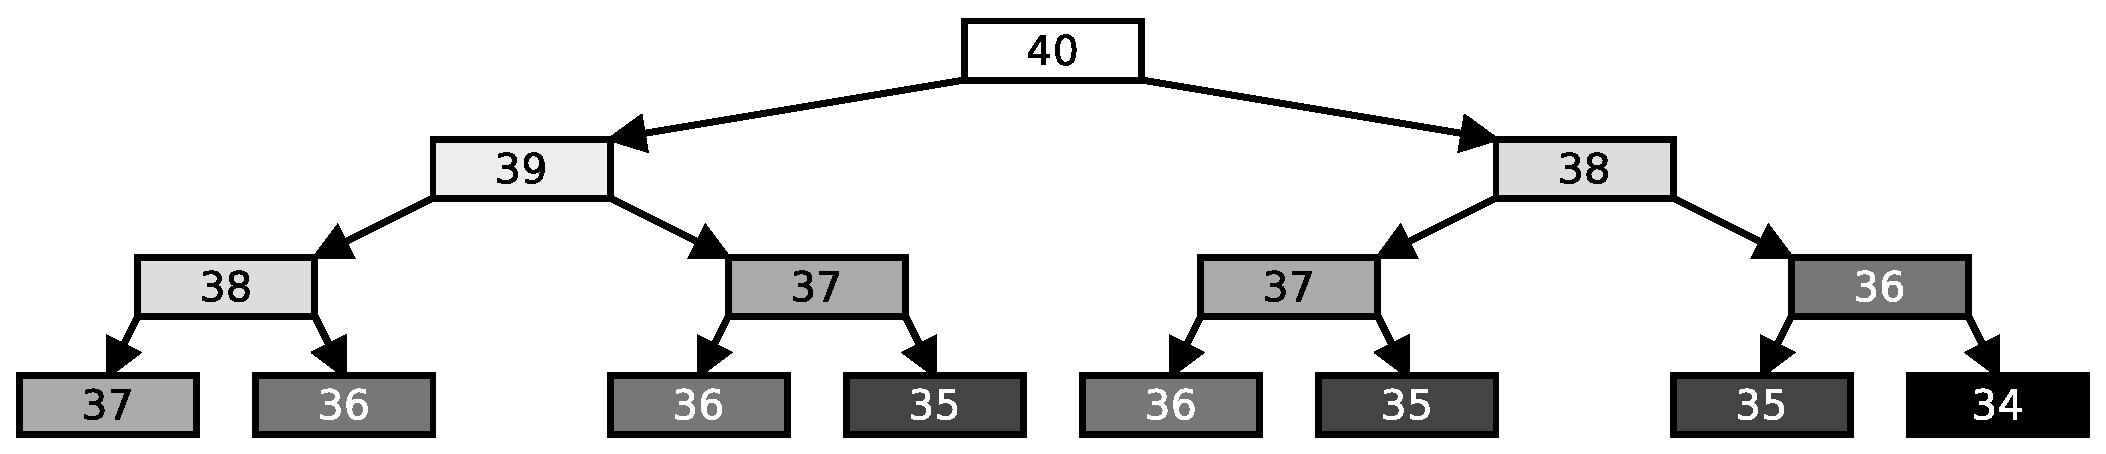
\includegraphics[width=\textwidth]{gfx/factorial-tree}
  \caption{Tree of recursive computations for the Fibonacci numbers. It can be observed that there are many repetitions. }
  \label{fig:fibotree}
\end{figure}

Not all is lost for recursive computation, however, because we can
very easily keep track of the values we have already calculated. If we
store these value in memory for later use we do not need to calculate
them again. We can use an array for this purpose, created the first
time the method is called. The resulting method could look like this: 

% NOTE: verified code
\begin{verbatim}
    // arrays are 0-based, so F(1) is stored at position 0, etc
    private int[] precalculated = null;

    public int fib(int n) {
        if (precalculated == null) {
           precalculated = new int[n];
           for (int i = 0; i < precalculated.length; i++) {
                precalculated[i] = -1; // to indicate "not calculated yet"
           }
        }
        if ((n == 1) || (n == 2)) {
          return 1; 
        } else {
            if (precalculated[n-1] != -1) {
                return precalculated[n-1];
            } else {
                int result = fib(n-1) + fib(n-2);
                precalculated[n-1] = result;
                return result;
            }
        }
    }
    // ...additional code would go here...
\end{verbatim}

This is kind of OK, but the clarity of this code could be greatly
improved with just two small tricks: first, move the initialisation
of the array to another method; second, remove the first \verb+if+ by
including the base cases (1 and 2) in the array at initialisation. The
new code would look like this: 

% Note: verified code
\begin{verbatim}
    // arrays are 0-based, so F(1) is stored at position 0, etc
    private int[] precalculated = null;

    // Fibonacci number are always positive
    private static final int UNKNOWN = -1;

    public int fib(int n) {
        if (precalculated == null) {
            initPrecalculatedArray(n);
        }
        if (precalculated[n-1] != UNKNOWN) {
            return precalculated[n-1];
        } else {
            int result = fib(n-1) + fib(n-2);
            precalculated[n-1] = result;
            return result;
        }
    }

    private void initPrecalculatedArray(int size) {
       precalculated = new int[size];
       for (int i = 0; i < precalculated.length; i++) {
            precalculated[i] = UNKNOWN;
       }
       precalculated[0] = 1; // F(1)
       precalculated[1] = 1; // F(2)
    }
    // ...additional code would go here...
\end{verbatim}

Now the method \verb+fib(int)+ is much clearer. If the array of
precalculated values is not initialised (i.e.~it is \verb+null+), we
initialise it. Then we start calculating smaller Fibonacci numbers and
storing them in the array. Before we do any calculation, we check the
array; if it contains the precalculated value, we just use that
number. There are no repeated calculations in this case. This version of the
method uses a couple of milliseconds for finding a Fibonacci number,
even for larger numbers. 

Storing intermediate variables for reusing them is a simple technique
called \emph{memoization} (not to be confused with memorization),
sometimes written memo-ization. 

The approach of solving a problem by dividing it into smaller
sub-problems, and combining the results of the smaller instances to
find the solution of the bigger one (memoizing intermediate results to
prevent redundant re-computation), is called \emph{dynamic
  programming}\footnote{It is important to note that (somewhat
  confusingly) the term ``dynamic programming'' has nothing to do with
  writing software, and actually \emph{predates} the appearance of
  computers and software by many years. 
  Originally, the term programming in 'dynamic programming'
  referred to ``program'' in the sense of a military schedule for
  training not in the sense of a list of instructions to be processed
  by a computer.}.

\section{Divide-and-conquer}
\label{sec:divide-conquer}

Some years ago, a guy called Julius Caesar conquered the Gaul in just
eight years; a remarkable feat at the time. He did not conquer the
whole Gaul in one go, but rather divided the problem (conquering the
Gaul) into smaller subproblems (conquering each small tribe) and then
solved the smaller problems to get to the final solution. 

We can use the same strategy in our programs. We can divide a problem
into smaller subproblems that we can attack more easily; once we have
the solution for the smaller subproblems, we can integrate those
solutions to get a general solution. This is called a
divide-and-conquer strategy and fits nicely with recursive
approaches. 

\subsection{More examples from the real world}
\label{sec:an-example-from}

Another example of divide-and-conquer in the real world (that, like
the Julius Caesar's example, seemed more interesting in the days before email
and twitter) is the postal mail system. The postal mail does not
deliver each letter individually, because that would be too
costly. Instead, the letters are roughly organised into zones, and then
sent in big lots to the zone offices to be delivered. Zone offices do not deliver
letters individually either, but assign them to areas or postal codes,
and send them in big batches to the right local post office. The local
post office is then able to deliver all letters in their area to their
final destinations. 

In the days of the internet, the Domain Name System is another example
of recursive divide-and-conquer. When you look for the server at
``www.bbk.ac.uk'', you start by asking the owner of the ``.uk''
domain. It does not have the address of every single machine in the
UK, but it knows which DNS servers are responsible of the top-level
subdomains (e.g.~co, ac, etc), so it can redirect you to the ``ac''
responsible. This server does not know every single machine in British
universities, but it knows who is responsible of each subdomain
(e.g.~bbk, ox, cam, etc), and will send you to the server responsible
of ``bbk''. This server can tell you what is the address of
``www.bbk.ac.uk'' so that you can access the homepage of Birkbeck. 

As you can see, dividing the problems of postal mail delivery and
domain name resolution into smaller subproblems makes them more
manageable. You have also observed that the smaller subproblems are
basically smaller versions of the big problem. This is the type of
situation in which recursive approaches come naturally. 

\subsection{Programming example: depth and size of a tree}
\label{sec:progr-exampl-depth}

A divide-and-conquer strategy is defined by three steps: 

\begin{enumerate}
\item Division of the big problem into two or more subproblems.
\item Finding the solution of the smaller subproblems.
\item Integration of the subsolution into a solution to the big
  problem. 
\end{enumerate}

We have already seen an example of a divide-and-conquer strategy. When
we calculated the depth of a binary tree, we did not need to iterate through
all the nodes in the tree counting steps as we traversed the tree up
and down. Instead, we divided the problem into two smaller
subproblems: finding the size of the left subtree and the right
subtree. Once we found the solution of both subproblems, the
integration involved taking the maximum depth and add one to it. 

A related problem is finding the size of a tree, i.e.~the number of
elements it contains. First, we divide the problem into two smaller
subproblems: finding the size of the left and right subtrees. Once we
get the solution to those problems, we can combine them by adding them
up plus one (for the root). Look at the following example with
additional comments marking the steps: 

\begin{verbatim}
    public int size() {
        // Step 1: Division of the problem into size-of-left and size-of-right
        int leftSize = 0
        if (left != null) {
            leftSize = left.size();
        }
        int rightSize = 0;
        if (right != null) {
            rightSize = right.size();
        }
        // Step 2: Integration of both subproblems
        int result = 1 + leftSize + rightSize;
        return result;
    }
\end{verbatim}


%%% Local Variables:
%%% mode: latex
%%% TeX-master: "d14"
%%% End:
